\BourbakiExercisesSection

\begin{enumerate}
\def\labelenumi{\arabic{enumi}.}
\item
  Give an example of a homomorphism \(\rho: \mathbf{A} \to \mathbf{B}\) of commutative rings and two A-modules E, F such that the canonical homomorphism (17) (no. 3) is neither injective nor surjective (cf.~§ 4, Exercise 2).
\item
  Give an example of a free A-module and a ring B such that the homomorphism (20) (no. 4) is not injective (§ 3, Exercise 3).
\item
  Give an example of a monogenous A-module E and a ring B such that the homomorphism (20) (no. 4) is not surjective (cf.~§ 4, Exercise 2).
\item
  Let \(\rho: A \to B\) be a ring homomorphism. For every A-module \(E\) , show that the diagram
\end{enumerate}

\pandocbounded{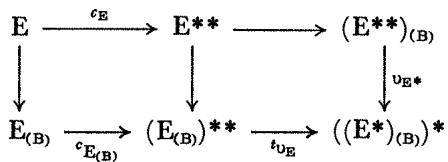
\includegraphics[keepaspectratio]{images/part003_7dd43288.jpg}}

is commutative.

\begin{enumerate}
\def\labelenumi{\arabic{enumi}.}
\setcounter{enumi}{4}
\item
  Let K be a field, A the product ring \(K^{N}\) , a the ideal \(K^{(N)}\) of A and B the ring A/a. Show that a is a projective A-module which is not finitely generated, although \(a_{(B)} = \{0\}\) .
\item
  With the rings A and B defined as in §1, Exercise 7, let M be an A-module; show that for M to be finitely generated (resp. free, projective), it is necessary and sufficient that \(M \otimes_{A} B\) be finitely generated (resp. free, projective).
\item
  Let \(\rho: A \to B\) be a ring homomorphism. For every left B-module \(F\) , define a canonical B-module homomorphism
\end{enumerate}

\[
\mathbf {F} \rightarrow \tilde {\rho} (\rho_ {*} (\mathbf {F}))
\]

and show that if E is a left A-module, the composite mappings

\[
\begin{array}{r l} & {\tilde {\rho} (\mathbf {E}) \to \tilde {\rho} (\rho_ {*} (\tilde {\rho} (\mathbf {E}))) \to \tilde {\rho} (\mathbf {E})} \\ & {\rho_ {*} (\mathbf {F}) \to \rho_ {*} (\tilde {\rho} (\rho_ {*} (\mathbf {F}))) \to \rho_ {*} (\mathbf {F})} \end{array}
\]

are the identity mappings.

